%%%%%%%%%%%%%%%%%%%%%%%%%%%%%%%%%%%%%%%%%
% Short Sectioned Assignment LaTeX Template Version 1.0 (5/5/12)
% This template has been downloaded from: http://www.LaTeXTemplates.com
% Original author:  Frits Wenneker (http://www.howtotex.com)
% License: CC BY-NC-SA 3.0 (http://creativecommons.org/licenses/by-nc-sa/3.0/)
%%%%%%%%%%%%%%%%%%%%%%%%%%%%%%%%%%%%%%%%%

% \documentclass[paper=a4, fontsize=11pt]{scrartcl} % A4 paper and 11pt font size
\documentclass[
	12pt,
	a4paper,
	english,
	spanish
]{scrbook}

% Images
\usepackage{eso-pic}

% Idioma
\usepackage[es-noindentfirst, es-lcroman, es-tabla]{babel}
%\spanishdashitems

% Titulo
\usepackage[
drafting=false,
dottedtoc=true,
parts,
pdfspacing,
beramono=false,
palatino=false,
%
floatperchapter=false,
linedheaders=true,
listings=false
]{notsoclassicthesis}

%\setsansfont[Scale=0.8]{Open Sans} 
%\renewfontface\chapterNumber[Scale=7, Color=000000]{EBGaramond}
%\setmonofont[Scale=0.75]{Go Mono}

% Matemáticas
\usepackage{amsmath, amsthm, amssymb}
\usepackage{mathtools}
\usepackage{commath}

% Teorema
\newtheoremstyle{theorem-style}  % Nombre del estilo
{\topsep}                                  % Espacio por encima
{\topsep}                                  % Espacio por debajo
{\itshape}                                  % Fuente del cuerpo
{0pt}                                  % Identación
{\scshape}                      % Fuente para la cabecera
{}                                 % Puntuación tras la cabecera
{5pt plus 1pt minus 1pt}                              % Espacio tras la cabecera
{\lsc{{\thmname{#1}\thmnumber{ #2}}.\thmnote{ (#3.)}}}  % Especificación de la cabecera
\theoremstyle{theorem-style}
\newtheorem{theorem}{Teorema}[section]
\newtheorem{corollary}[theorem]{Corolario}
\newtheorem{lemma}[theorem]{Lema}
\newtheorem{proposition}[theorem]{Proposición}
\newtheorem{question}{Pregunta}
\newtheorem{conjecture}[theorem]{Conjetura}
\newtheorem{remark}[theorem]{Nota}
\newtheoremstyle{definition-style}  % Nombre del estilo
{\topsep}                                  % Espacio por encima
{\topsep}                                  % Espacio por debajo
{}                                  % Fuente del cuerpo
{0pt}                                  % Identación
{}                      % Fuente para la cabecera
{.}                                 % Puntuación tras la cabecera
{5pt plus 1pt minus 1pt}                              % Espacio tras la cabecera
{\lsc{{\thmname{#1}\thmnumber{ #2}}\thmnote{ (#3)}}}  % Especificación de la cabecera
\theoremstyle{definition-style}
\newtheorem{definition}[theorem]{Definición}
\newtheorem{example}[theorem]{Ejemplo}
\newtheorem{notation}[theorem]{Notación}
\newtheorem{exercise}[theorem]{Ejercicio}


% Listas
\usepackage[inline]{enumitem}
\setlist[itemize]{ noitemsep, leftmargin=*}
\setlist[enumerate]{noitemsep, leftmargin=*}

% Posicionamiento
\usepackage{float}

% Código
\usepackage{listings}
\lstset{
	basicstyle=\ttfamily,%
	breaklines=true,%
	captionpos=b,                    % sets the caption-position to bottom
	tabsize=2,	                   % sets default tabsize to 2 spaces
	frame=none,
	numbers=left,
	xleftmargin=18pt,
	stepnumber=1,
	aboveskip=12pt,
	showstringspaces=false,
	keywordstyle=\bfseries,
	commentstyle=\itshape,
	numberstyle=\scriptsize\bfseries,
	morekeywords={sage},
}
\renewcommand{\lstlistingname}{Listado}

\usepackage{cite} %para incluir citas del archivo <nombre>.bib

% Lorem
\usepackage{blindtext}


\begin{document}

	% Plantilla portada UGR
	\begin{titlepage}
\newlength{\centeroffset}
\setlength{\centeroffset}{-0.5\oddsidemargin}
\addtolength{\centeroffset}{0.5\evensidemargin}
\thispagestyle{empty}

\noindent\hspace*{\centeroffset}

	
\includegraphics[width=0.9\textwidth]{logos/logo_ugr.jpg}\\[1.4cm]

	\begin{addmargin}[2.56cm]{0cm}
		\begin{minipage}{\textwidth}
			\textsc{\bfseries E.T.S de Ingenierías Informática y de Telecomunicación}\\
			
			\textsc{GRADO EN INGENIERÍA INFORMÁTICA}
			
			\vspace{3.0cm}
			
			\spacedlowsmallcaps{TRABAJO FIN DE GRADO}\\[0.5cm]
			\begingroup
				\LARGE{\bfseries Funciones de distancia con signo}\\\bigskip
			\endgroup
	
			\vspace{3.0cm}
			
			\large{Autor.\\ Lukas Häring García}\\[0.4cm]
			\large{Director.\\ Juan Carlos Torres Cantero}\\[2cm]
			%
\includegraphics[width=0.3\textwidth]{logos/etsiit_logo.png}\\[0.1cm]
			\textsc{---}\\
			%Granada, Junio de 201x
			Granada\\
			Curso académico 2019-2020
		\end{minipage}
	\end{addmargin}

\end{titlepage}


	% Plantilla prefacio UGR
	\thispagestyle{empty}

\chapter*{Resumen}

Gracias al rápido avance tecnológico y la evolución de la unidad de procesamiento de gráficos o \textit{GPU}, podemos experimentar con técnicas propuestas durante el siglo pasado, que eran poco eficientes debido al hardware del momento. El objetivo de este trabajo es hacer uso de este avance para probar nuevas técnicas de creación de escenas, utilizando una clase de funciones, conocidas como \textit{Funciones de distancia con signo} o \textit{FDS}\ref{ch:fds}. Desarrollaremos el proyecto en el lenguaje \textit{GLSL}\ref{ch:glsl}, donde veremos alguno de los nuevos tipos y operadores ya que es su sintaxis es similar a C. Las escenas creadas a partir de las \textit{Funciones de distancia con signo} son completamente analíticas, es decir, exactas, que a diferencia de otras técnicas que utilizan vértices. Por ejemplo, estas otras técnicas generan una esfera aproximada por un poliedro geodésico\footnote{Se trata de un poliedro convexo hecho de triángulos, el algoritmo: \url{https://stackoverflow.com/a/17795311}}. Para el renderizado de la escena tridimensional, en el cuarto capítulo, presentaremos un algoritimo con el nombre de \enquote{\textit{Spheremarcher}}\ref{sec:spheremarching}.

\vspace{0.7cm}

\noindent{
	\spacedlowsmallcaps{Palabras clave}
	\textit{gráficos}, \textit{marcher}, \textit{GLSL}, \textit{modelo de iluminación}
}

\cleardoublepage

\chapter*{Summary}

\begin{otherlanguage}{english}
In this project we are going to present a new graphic technique in thanks to the advance in technology and the continuously increasing of the efficiency of the GPU. We are going to divide it into five important chapters.

\paragraph{Chapter 1} In this first chapter we are going to present the mathematical foundation used to create an analytical scene for our project. We will give an introduction to the \textit{signed distance functions} and dive into them in later chapters. Because we are working with analytical scenes, we will present a theorem to calculate surface normal that will be in the Light Model. Finally, we will give two mathematical concepts: \textit{homeomorphism} and \textit{homotopies}, commonly used in textures.

\paragraph{Chapter 2} In this second chapter, we will present the language we will use through the whole project, called \textit{GLSL}. The syntax of this language is similar to C, we will be presenting some new mathematical types and primitive functions. Each section will also have tips and code examples.

\paragraph{Chapter 3} In this chapter we will analyze the analytical algorithm used to approximate a sceene that is created using \textit{signed distance functions}. We will be presenting the online enviroment used to create this project, called \textit{Shadertoy}, designed by Iñígo Quilez and Pol Jeremias in 2013.

\paragraph{Chapter 4} In this chapter, we will be presenting the basic operators to create an Illumination Model. We are going to implement an Illumination Model designed in the 70's, called Phong's Model. This model splits the light intensity into three different ones: ambient intensity, that affects with a constant value at the surface everywhere; diffuse intensity, dependent to the surface curvature and the light direction; finally, specular intensity is calculated by the reflection of the light from the surface to the eye.

\paragraph{Chapter 4} In this chapter we will be covering the main theme of this project, that are indispensable for the creationg of a sceene. \textit{Signed distance functions} are a special type of functions that returns a signed distance to a surface or perimetre, when the distance is positive, we would say that we are outside the sceene, when it is negative, we will be inside an object. The zeros will represent the surface but because we will be using an numerical 

\vspace{0.7cm}
\noindent{
	\spacedlowsmallcaps{Keywords}
	\textit{open source}, 
	\textit{floss}
}

\end{otherlanguage}

\cleardoublepage
%\thispagestyle{empty}
%\noindent\rule[-1ex]{\textwidth}{2pt}\\[4.5ex]
%D. \textbf{Tutora/e(s)}, Profesor(a) del ...
%\vspace{0.5cm}
%\textbf{Informo:}
%\vspace{0.5cm}
%Que el presente trabajo, titulado \textit{\textbf{Chief}},
%ha sido realizado bajo mi supervisión por \textbf{Estudiante}, y autorizo la defensa de dicho trabajo ante el tribunal
%que corresponda.
%\vspace{0.5cm}
%Y para que conste, expiden y firman el presente informe en Granada a Junio de 2018.
%\vspace{1cm}
%\textbf{El/la director(a)/es: }
%\vspace{5cm}
%\noindent \textbf{(nombre completo tutor/a/es)}

%\chapter*{Agradecimientos}





	% Índice de contenidos
	%\newpage
	%\tableofcontents
	{\hypersetup{hidelinks}
		\tableofcontents
	}

	% Índice de imágenes y tablas
	%\newpage
	%\listoffigures

	% Si hay suficientes se incluirá dicho índice
	%\listoftables 
	%\newpage

	% Introducción 
	\chapter{Preliminares}


% https://it.wikipedia.org/wiki/Isosuperficie#cite_note-:2-3
\section{Funciones de distancia con signo\label{sec:fds}}

Una función de distancia con signo (\textit{FDS}) se trata de una aplicación \(f: \mathbb{R}^n\longrightarrow \mathbb{R}\). Esta aplicación transforma un punto \(\Vec{p}\) de un espacio multidimensional en un valor. En particular, trabajaremos con espacios bidimensionales y tridimensionales, donde el valor devuelto es la distancia mínima con signo hasta un punto \(\Vec{q}\) de un perímetro o una superficie \(S\). 
\[f(\Vec{p})=\pm min_{\Vec{q}\in S}\vert\vert \Vec{p}-\Vec{q} \vert\vert , \Vec{p} \in \mathbb{R}^n, n\in \{2,3\}\]
El signo de esta distancia contiene información sobre la escena: con una distancia positiva, nos encontramos en el exterior de una figura, en caso de ser cero, nos encontraremos en la superficie (corteza) \(S\), por último, con una distancia negativa, estaremos dentro del volúmen de la figura, que en positivo representa la profundidad del punto respecto de la corteza \cite{hart1996sphere}. 

\begin{definition}
	Sea \(f:\mathbb{R}^2\longrightarrow\mathbb{R}\), una función de distancia con signo, definimos como \textit{isoperímetro}, \(L=\{\Vec{p} \vert f(\Vec{p})=0\}\).
\end{definition}

\begin{definition}
	Sea \(f:\mathbb{R}^3\longrightarrow\mathbb{R}\), una función de distancia con signo, definimos como \textit{isosuperficie}, \(S=\{\Vec{p} \vert f(\Vec{p})=0\}\).
\end{definition}

Para esta última definición, presentaremos un algoritmo de trazado de escena denominado \textit{Spheremarcher}\ref{sec:spheremarching}.
\newpage
\section{La normal de una isosuperficie \label{sec:normal}}

Vamos a presentar un teorema esencial para el cálculo de la normal de una superficie, cuya demostración propuesta por  \cite{goldman2005curvature} (p. 641-642). Esta es fundamental para la confección de una escena, especialmente en un modelo de iluminación\ref{ch:iluminacion}.

\begin{theorem}
	El vector gradiente \(\nabla f(x_0, y_0, z_0)\)  es perpendicular a la curva de la tangente de una \textit{isosuperficie} en el punto \(\Vec{p}=(x_0, y_0, z_0)\).
\end{theorem}

En realidad, nos quiere decir que la normal de una \textit{isosuperficie} es proporcional a su gradiente o exacta en caso de su posterior normalización\footnote{Decimos que un vector está normalizado cuando su módulo es exactamente \(1\) .}, que denotaremos:
\[norm:\mathbb{R}^n\longrightarrow\mathbb{R}^n, norm(\Vec{v})=\dfrac{\Vec{v}}{\vert\vert v \vert\vert}\]
%Su demostración está basada en el concepto del plano tangente.\\\\
% https://tutorial.math.lamar.edu/classes/calciii/gradientvectortangentplane.aspx
Se define formalmente el gradiente de una función tridimensional, como:
\[ \nabla f(x, y, z)= < \partial_x f, \partial_y f, \partial_z f, > \]
donde \enquote{\(\partial_{x_i}\)} es la derivada parcial de una función respecto de la variable \(x_i\). Definida por: 
\[ \partial_{x_i}f=\lim_{\epsilon\longrightarrow 0}\dfrac{f(x_0,\cdots,x_i+\epsilon,\cdots,x_n)-f(x_0, \cdots, x_n)}{\epsilon} \]
Se puede aproximar computacionalmente, tomando \(\epsilon\) próximo a \(0\), por ejemplo, \(\epsilon = 0.001\).
Finalmente, definimos el gradiente computado como:
\[
\Vec{n}=norm(\nabla f(x, y, z))\approx norm\left(
\stretchleftright[1000]{\langle}
{\begin{array}{c}
\dfrac{f(x+0.001,y,z)-f(x,y,z)}{0.001}\\
\dfrac{f(x,y+0.001,z)-f(x,y,z)}{0.001}\\
\dfrac{f(x,y,z+0.001)-f(x,y,z)}{0.001} \end{array}}
{\rangle}\right)
\]

\section{Homeomorfismos sobre [0, 1]}

Vamos a definir una aplicación que nos ayudará a deformar funciones de manera continua. Esta aplicación nos será muy útil para manipular las propiedades de la escena, por ejemplo, la intensidad lumínica en nuestro modelo de iluminación, transformación de color, velocidad de un objeto de un punto a otro, etc.

\begin{definition}
    Sea una función \(f:X\longrightarrow Y\), diremos que esta es homeomórfica, si y solo si:
    \begin{enumerate}
        \item \(f\) es continua.
        \item \(f\) es biyectiva.
        \item \(f^{-1}\) es continua.
    \end{enumerate}
\end{definition}
Restringimos los homeomorfismos a \(X=Y=[0,1]\) con \(f(0)=0\) y \(f(1)=1\). Esta restricción es importante para valores normalizados, ya que aseguramos que sus extremos quedan invariantes.\\\\
Supongamos una imagen en escala de grises con un único canal. El canal acepta un intervalo real \([0, 1]\), donde el color negro es el \(0\) y el blanco, el \(1\). Por ejemplo, definimos nuestro \textit{homeomorfismo}:
\[f(x)=x^8, x \in [0, 1]\]
Así, podemos comprobar que esta función cumple con las propiedades descritas anteriormente. En la siguiente representación podemos distinguir una serie de exponentes desde 1 hasta 11, en \textcolor{blue}{azul} nuestra función \(f\).
\begin{figure}[H]
    \centering
    \captionsetup{justification=centering}%,margin=2cm
    \begin{tikzpicture}[scale=0.8]
        \begin{axis}[
            % Function Properties
            domain=0:1,
            samples=100,
            % Grid Properties
            grid=both,
            % X, Y Coordinates
            axis lines=left,
            compat=newest,
            xlabel=$x$, xlabel style={at={(1,0)}, anchor=west},
            ylabel=$y$, ylabel style={rotate=-90,at={(0,1)}, anchor=south}
        ]
            \addplot[gray] (x,x);
            \addplot[gray] (x,x^2);
            \addplot[gray] (x,x^3);
            \addplot[gray] (x,x^4);
            \addplot[gray] (x,x^5);
            \addplot[gray] (x,x^6);
            \addplot[gray] (x,x^7);
            \addplot[blue, very thick] (x,x^8);
            \addplot[gray] (x,x^9);
            \addplot[gray] (x,x^10);
            \addplot[gray] (x,x^11);
        \end{axis}
    \end{tikzpicture}
    \caption{Gráfica de los distintos \(f_n(x)=x^n, n\in\{1,\cdots,11\}\subset \mathbb{N}\) } \label{fig:M1}
\end{figure}
Los valores inferiores a \(0.6\) se transforman a valores próximos a \(0.0\), oscureciendo los tonos grises, manteniendo los colores claros.
\begin{figure}[H]
  \centering
  \captionsetup{justification=centering}%,margin=2cm
  \subfloat[Imagen original]{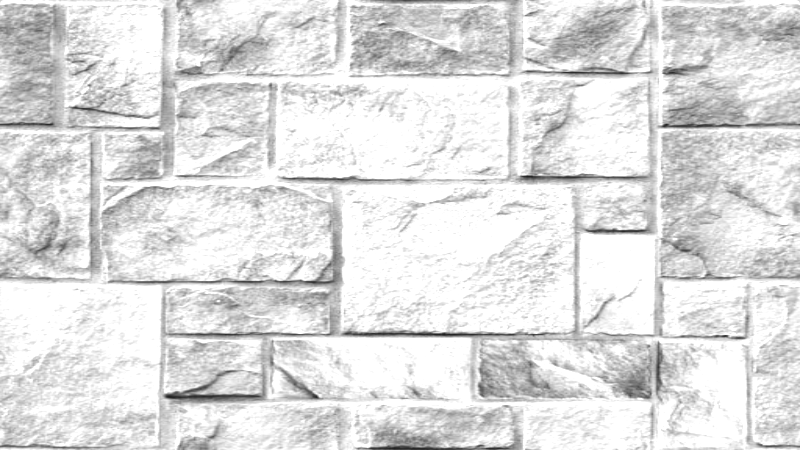
\includegraphics[width=0.45\textwidth]{secciones/imagenes/preliminars/pol8-img-left.png}}
  \hfill
  \subfloat[\(f(x)=x^8\) sobre la imagen original]{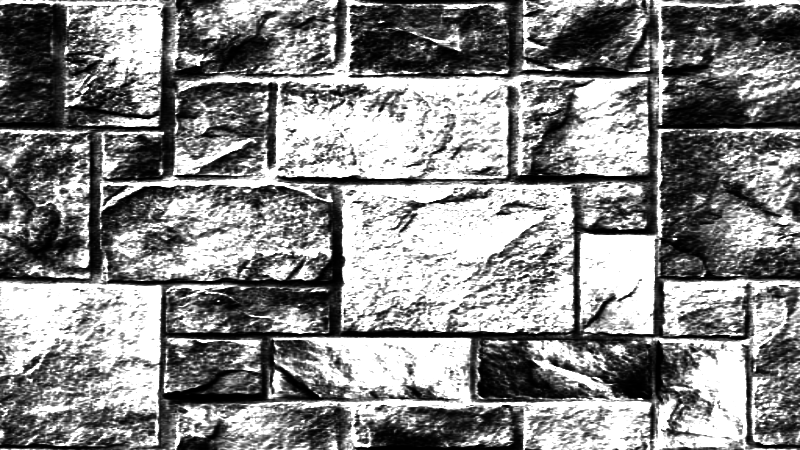
\includegraphics[width=0.45\textwidth]{secciones/imagenes/preliminars/pol8-img-right.png}}
  \caption{A la izquierda una imagen con un canal \([0,1]\). A la derecha, la misma imagen, pero aplicado el \textit{homeomorfismo} \(f\).}
  \label{fig:homeomorphism}
\end{figure}
En código: \url{https://www.shadertoy.com/view/wljfR1}

\section{Homotopías}
% Nota pie
En esta última sección, vamos a ver una aplicación matemática que es utilizada para animación y texturización. Vamos a centrarnos en el intervalo \([0, 1]\), aunque podemos trabajar sobre cualquier intervalo, antes deberemos normalizar y  finalmente, reescalar.

\begin{definition}
    Dadas dos aplicaciones \(f, g:X\longrightarrow Y\), continuas, decimos que son homotópicas. Si existe una aplicación \(H\), también continua, tal que:
    \[ H:X\times[0,1]\longrightarrow Y \]
    \[ H(x, 0)=f(x) \]
    \[ H(x, 1)=g(x) \]
\end{definition}
% nota pie
\begin{definition}
    Claramente \(H\) es una homotopía, llamaremos función de mezcla lineal\label{def:mix}\footnote{Se utiliza este concepto en la documentación oficial, sección \enquote{8.3 Common Functions}} a la homotopía:
    \[H(x, t)=(1-t)\cdot f(x) + t\cdot g(x)\]
\end{definition}

Como podemos observar,  la última definición es una homotopía, ya que, la suma de dos funciones continiuas es siempre continua y los extremos resultan \(f(x)\) y \(g(x)\), respectivamente.\\\\
Como \(t\in[0,1]\), podemos aplicar un \textit{homeomorfismo} \(p(t)\) y tener así, una versión más general.
    \[H(x, t')=H(x, p(t))=(1-p(t))\cdot f(x) + p(t)\cdot g(x)\]
Veamos un ejemplo, supongamos que \(f(x)\) y \(g(x)\) son los colores de una imagen 3-canal y como \(t\), una tercera imagen con un canal \([0,1]\), que actuará como máscara.
\begin{figure}[H]
  \centering
  \captionsetup{justification=centering}%,margin=2cm
  \subfloat[Imagen \(f(x)\)]{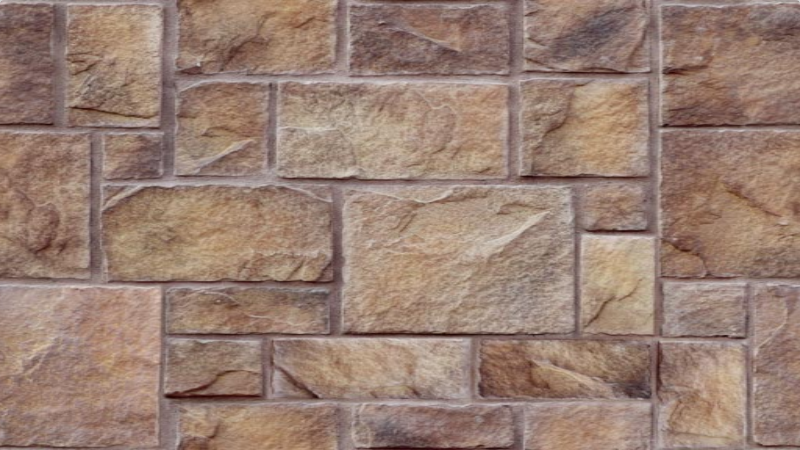
\includegraphics[width=0.30\textwidth]{secciones/imagenes/preliminars/texture-wall.png}}
  \hfill
  \subfloat[Imagen \(g(x)\)]{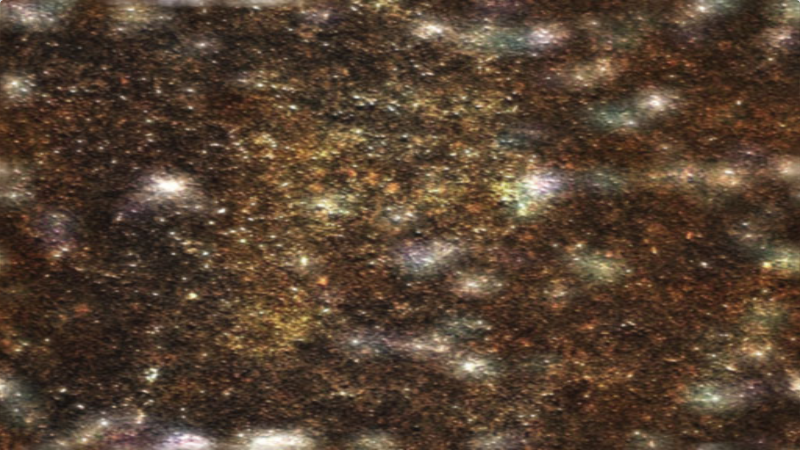
\includegraphics[width=0.30\textwidth]{secciones/imagenes/preliminars/texture-galaxy.png}}
  \hfill
  \subfloat[Máscara \(t\)]{
\includegraphics[width=0.30\textwidth]{secciones/imagenes/preliminars/mask.png}}
  \caption{Imagen \(f(x)\), Imagen \(g(x)\) y Máscara \(t\)}
  \label{fig:textures}
\end{figure}
Los resultados obtenidos con diferentes homomorfismos.
\begin{figure}[H]
  \centering
  \captionsetup{justification=centering}%,margin=2cm
  \subfloat[Mezcla con el homeomorfismo \(p(t)=t\)]{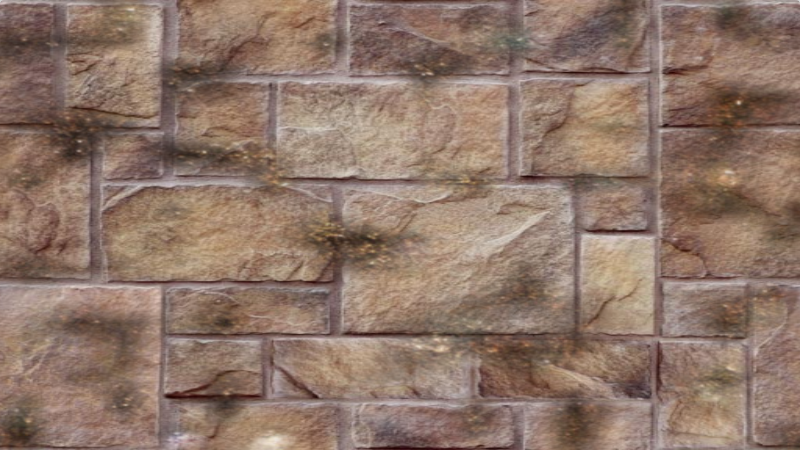
\includegraphics[width=0.45\textwidth]{secciones/imagenes/preliminars/masking-result-1.png}}
  \hfill
  \subfloat[Mezcla con el homeomorfismo \(p(t)=t^4\)]{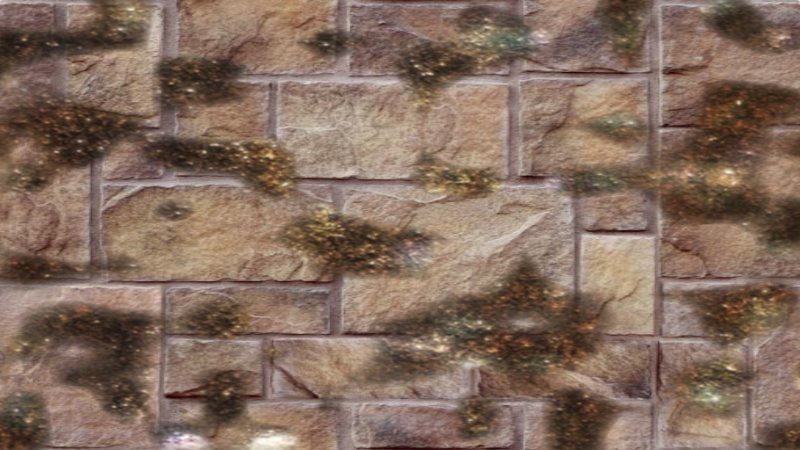
\includegraphics[width=0.45\textwidth]{secciones/imagenes/preliminars/masking-result-2.png}}
  \caption{Mezcla con distintos homomorfismos.}
  \label{fig:homotopies}
\end{figure}

Un ejemplo práctico: \url{https://www.shadertoy.com/view/wt2fR1}

	% Descripción del problema y hasta donde se llega
	\chapter{Descripción del problema}



	% Estado del arte
	% 	1. Crítica al estado del arte
	% 	2. Propuesta
	\chapter{Estado del arte}


	
	\chapter{Planificación}

\section{Metodología utilizada}


\section{Temporización}

\section{Seguimiento del desarrollo}


	% Análisis del problema
	% 1. Análisis de requisitos
	% 2. Análisis de las soluciones
	% 3. Solucion propuesta
	% 4. Análisis de seguridad
	\chapter{Análisis del problema}
 


	% Desarrollo bajo sprints: 
	% 	1. Permitir registros y login de usuarios
	% 	2. Desarrollo del sistema de incidencias
	% 	3. Desarrollo del sistema de denuncias administrativas y accidentes
	% 	4. Desarrollo del sistema de croquis
	%   5. Instalación de la aplicación de manera automática
	\chapter{Implementación}



	% Presupuesto

	% Conclusiones
	\chapter{Conclusiones y trabajos futuros}



	% Trabajos futuros


	
	\newpage
	\bibliography{bibliografia}
	\bibliographystyle{plain}
	
\end{document}

